%%
%% Implementation
%%

\chapter{Implementation}

Thist chapter \ldots

\section{System Overview}

Figure~\ref{fig:SystemOverview} presents an overview of the complete system containing
one simulated \ac{RV} and the ground station.

The simulated \ac{RV} mainly comprises an Apache Tomcat web container, which executes a
Pilot web pplication and an Engine web application.
%
The Pilot web application consists of model helicopter plant simulator, that is, the MockJAviator,
a flight control system, an auto pilot, and a sensor simulator.
The MockJAviator emulates the helicopter's flight dynamics and \ac{IMU},
the flight control system operates attitude and altitude of the simulated vehicle, 
and the autopilot stirs the simulated vehicle along a \ac{VCL} script defined trajectory.
The sensor simulator supports GPS reveivers, belly mounted cameras, thermometers, barometers,
and sonar sensors.
\begin{figure}[h]
	\begin{center}
		{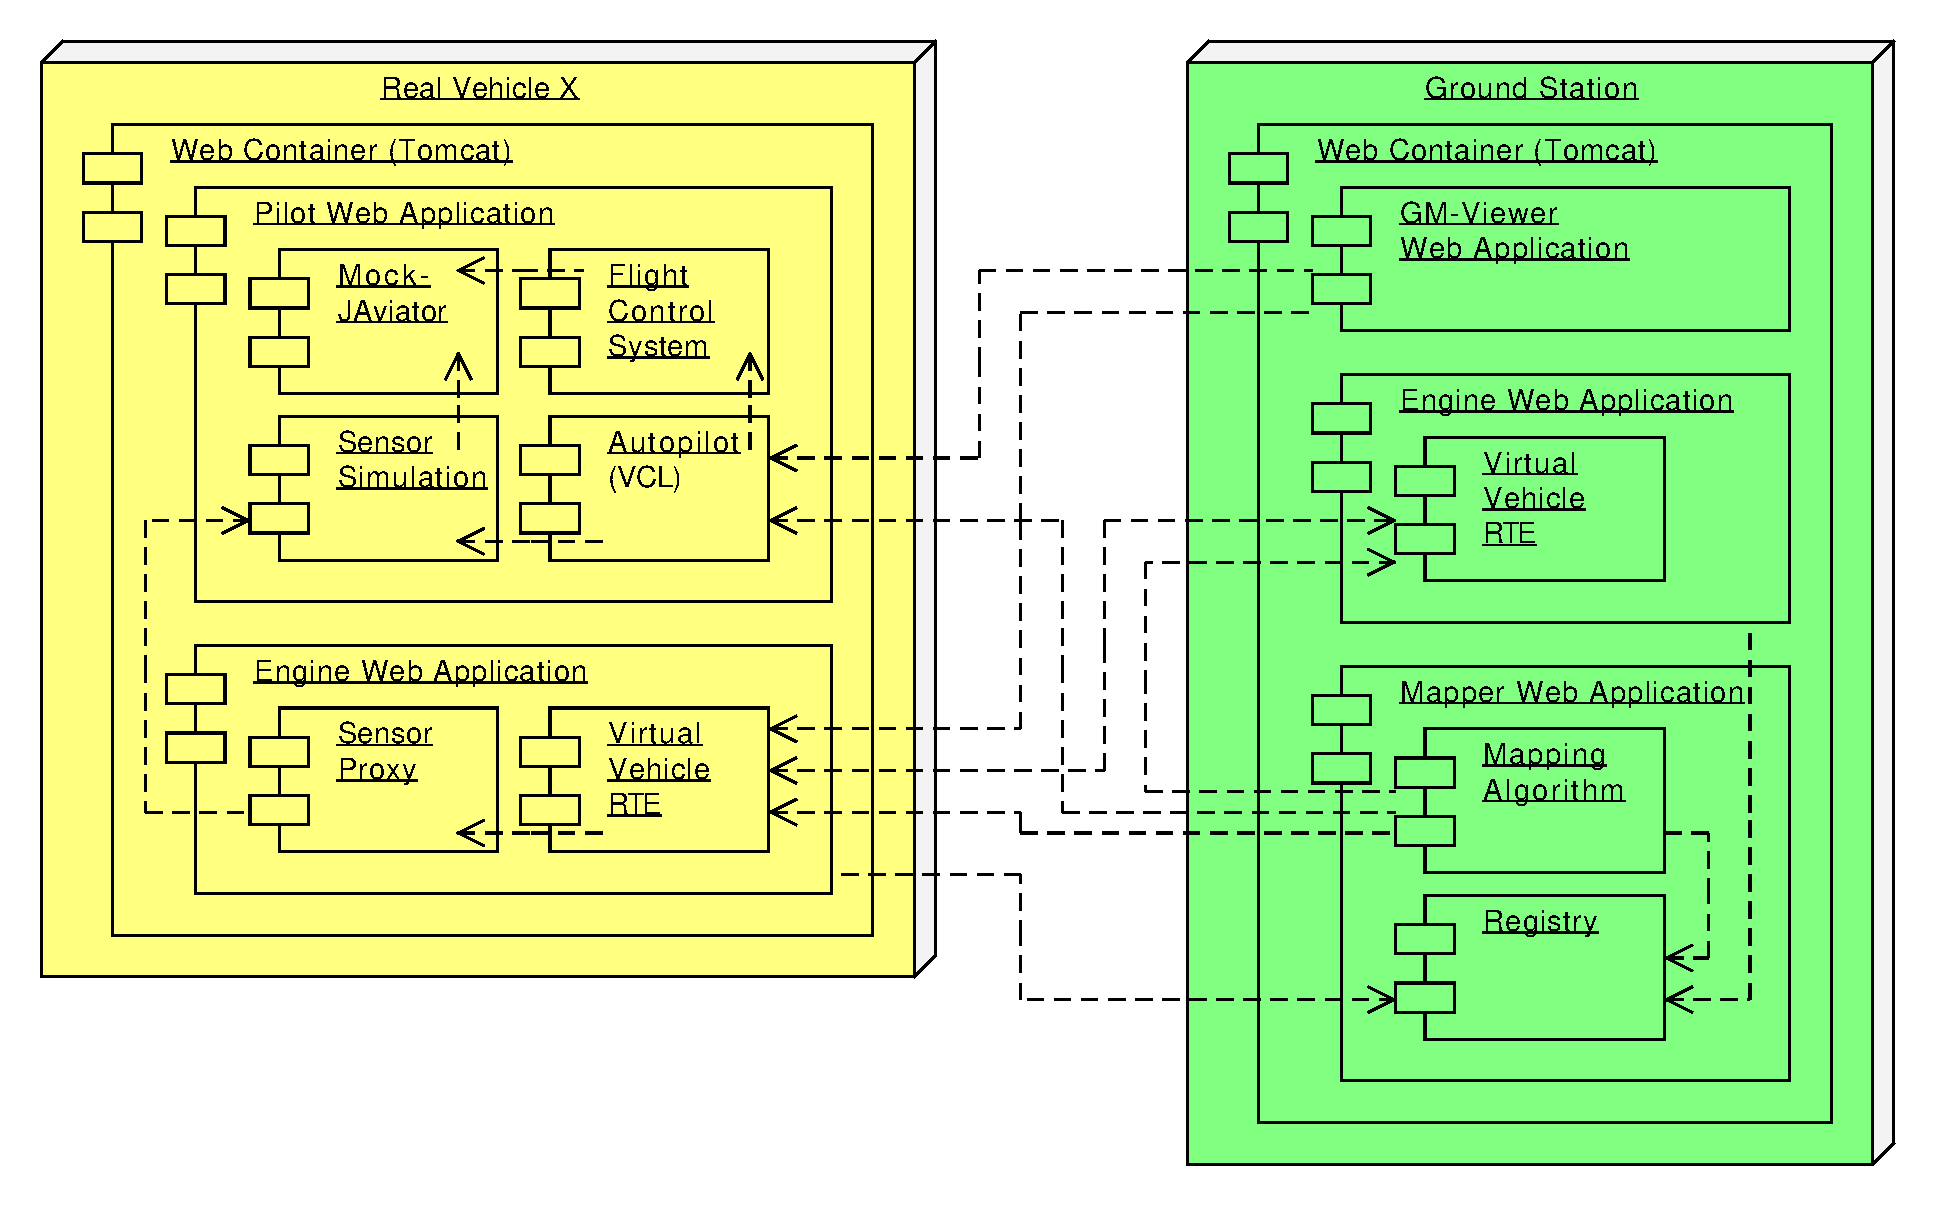
\includegraphics[width=10cm]{SystemOverview.pdf}}
	\end{center}
	\caption{System Overview.\label{fig:SystemOverview}}
\end{figure}

The ground station executes an Apache Tomcat web container, which runs a Google Maps Viewer
web application, a Engine web application, and a Mapper web application.
%
The Google Maps Viewer web application allows an operator to supervise ongoing missions.
%
The ground station Engine web application provides a \ac{VV RTE} for uploading and downloading \acp{VV}. 
%
Registry and mapping algorithm are the main components of the Mapper web application.
The mapping algorithm assigns \acp{VV} to \acp{RV}, based on fight plans and available sensors.
%
Each Engine web application registers with the Mapper's registry.


\section{Sensor Simulation}
Figure~\ref{fig:SensorSimulation} visualizes the simulation of sensors.
%
The current implementation supports belly mounted cameras, random number generators for emulating thermometers and
barometers, GPS position sensors, and sonar sensors.

 
\begin{figure}[h]
	\begin{center}
		{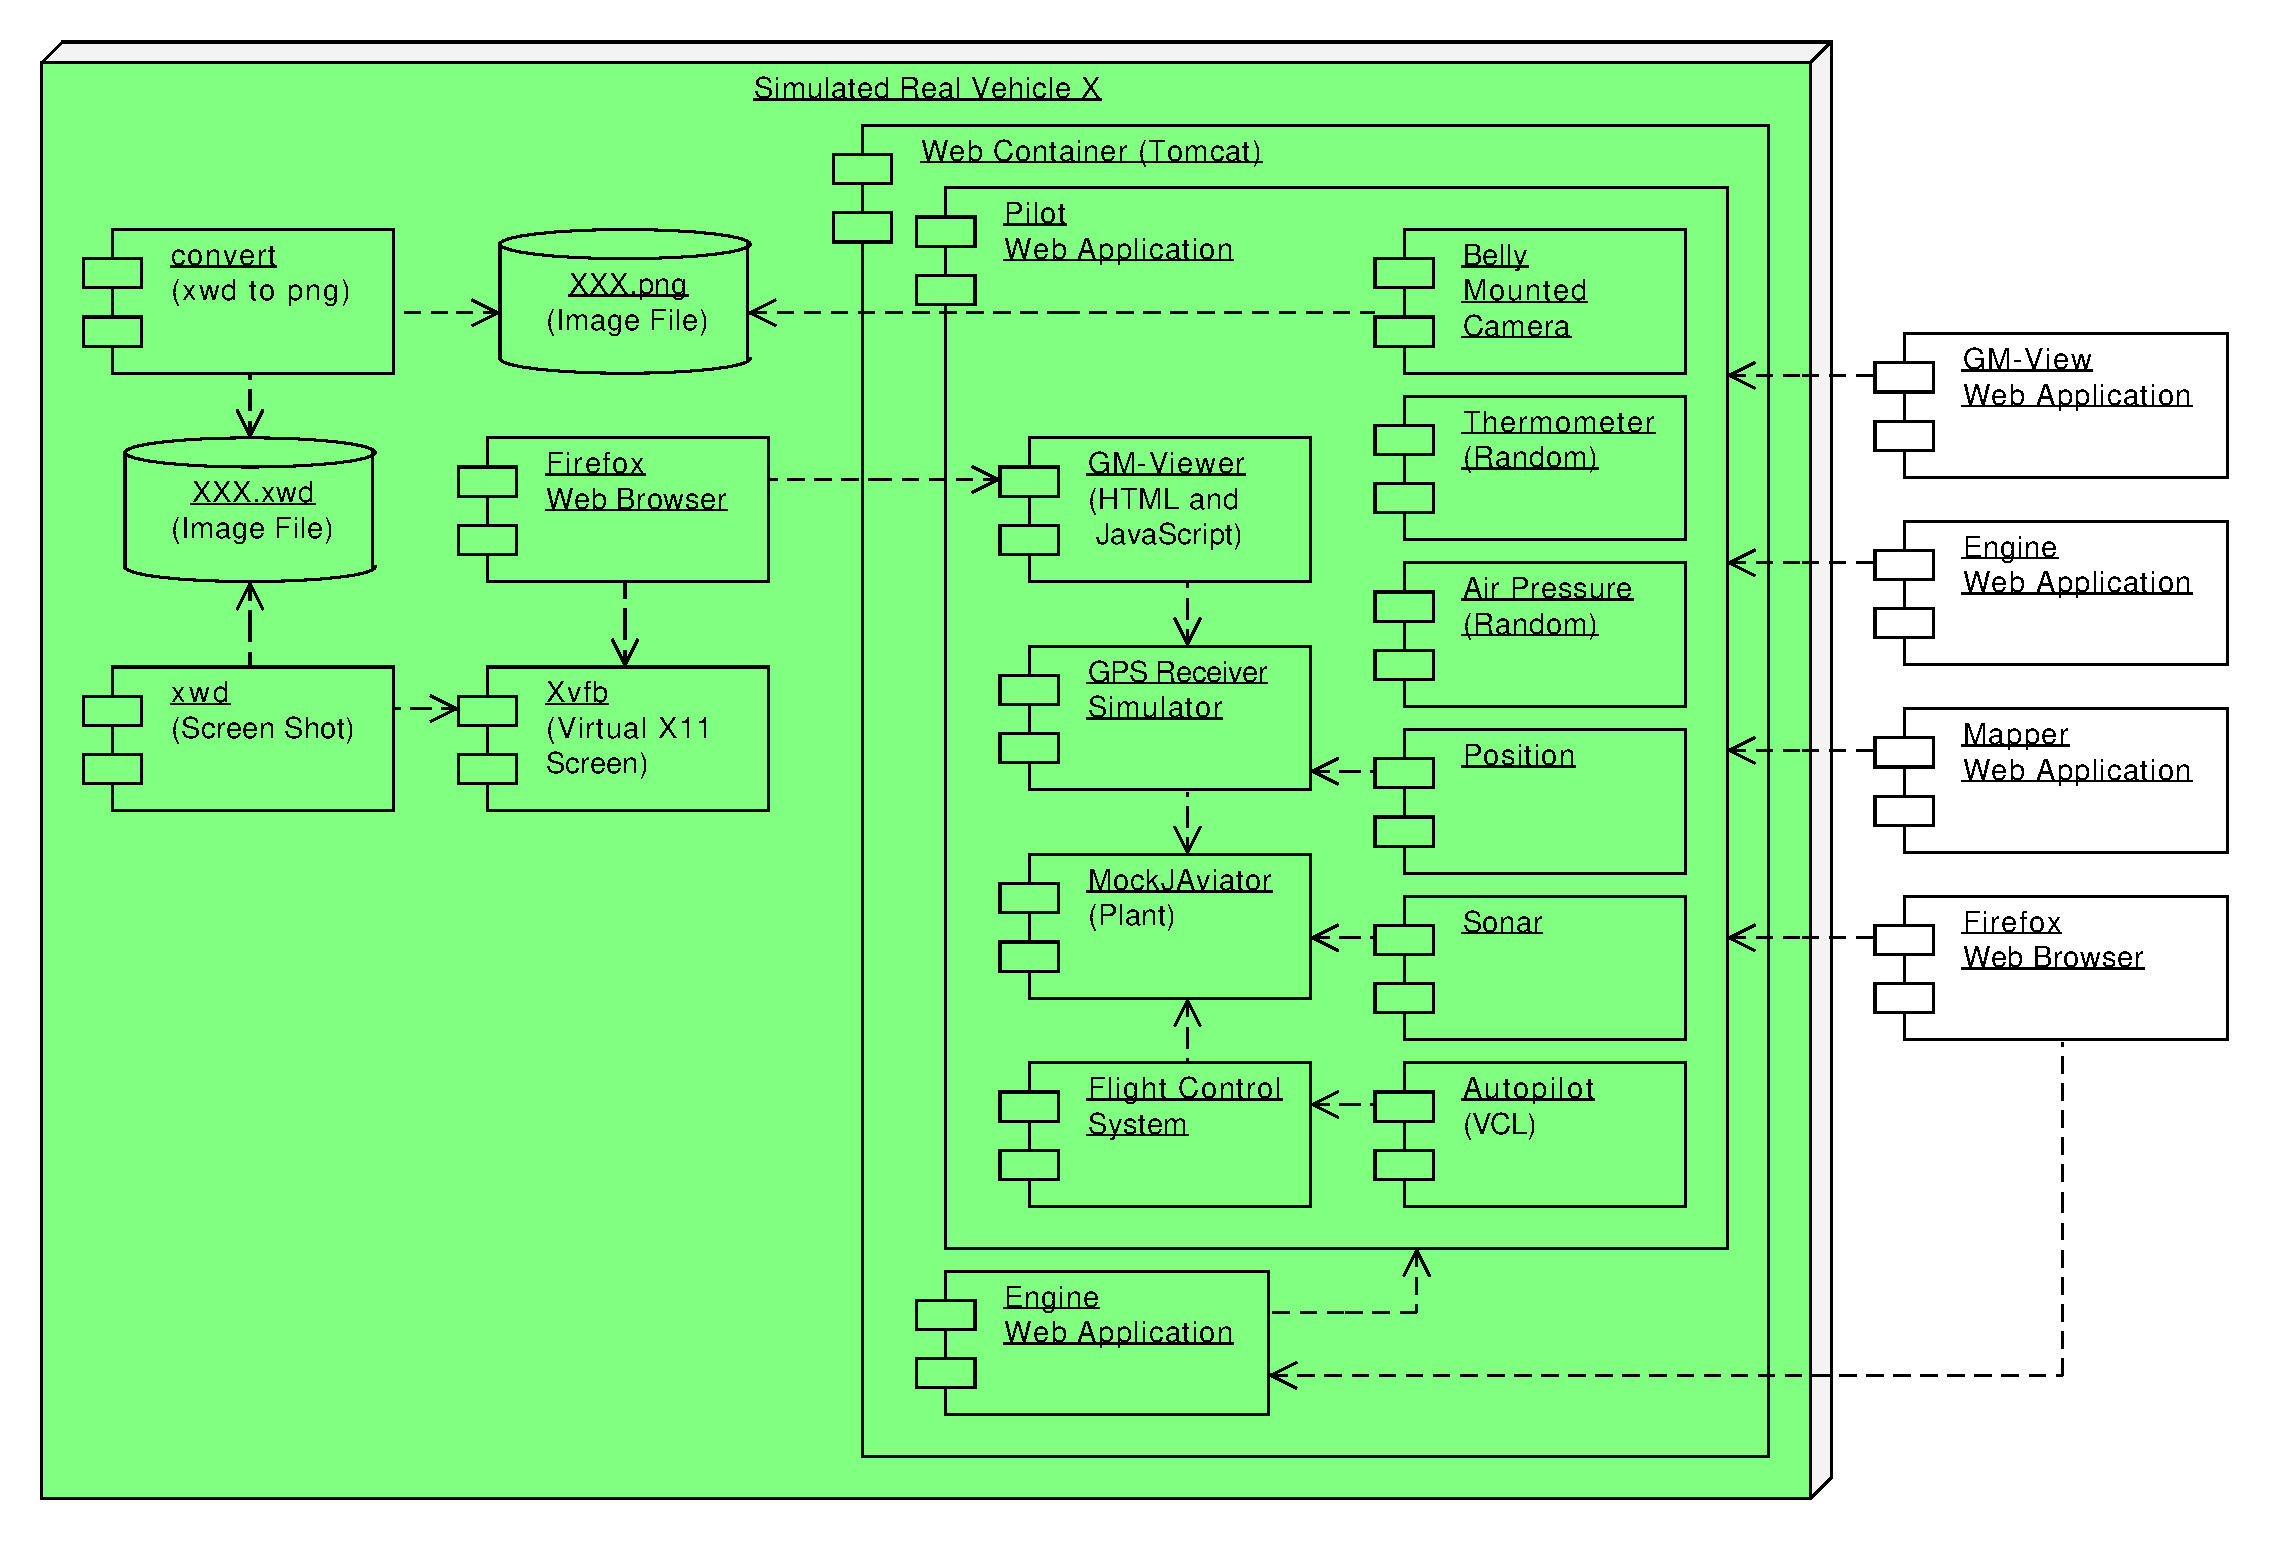
\includegraphics[width=11.6cm]{SensorSimulation-3.pdf}}
	\end{center}
	\caption{Sensor Simulation.\label{fig:SensorSimulation}}
\end{figure}


The belly mounted camera delivers a Google Maps satellite image indicating the position of the simulated vehicle by a
visual marker, exemplified by Figure~\ref{fig:BellyMountedCamera}.
To achieve this, the Pilot web application supplies a JavaScript enhanced HTML page.
\begin{figure}[h]
	\begin{center}
		{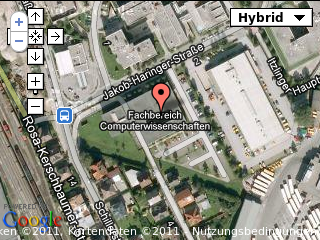
\includegraphics[width=6cm]{bmc-photo-cosy.png}}
	\end{center}
	\caption{A photo captured by the belly mounted camera.\label{fig:BellyMountedCamera}}
\end{figure}

Once the Firefox web browser selects this page, the embedded JavaScript program periodically polls the Pilot web
application for the vehicle's current position. After that, the JavaScript program slides the center of the
displayed satellite view to this position and repositions the marker.
To allow several belly mounted cameras beeing simulated on the same machine, the utilized web browsers use \ac{Xvfb}
devices as output screens.
%
Whenever the belly mounted camera needs to deliver a photo, it applies the \texttt{xwd} utility to take a snapshot
of the corresponding \ac{Xvfb} device, converts this snapshot to an image in PNG format by using program
\texttt{convert}, and delivers it via \ac{HTTP}.

Thermometer and air pressure sensors apply random number generators to simulate values.
The position sensor queries the GPS receiver simulator for the current position of the vehicle, and the sonar
sensor reads the current altitude over ground from the instantiated MockJAviator.

\section{Configuration}
This section covers the configuration of the web applications Pilot, Engine, Mapper, and GM-Viewer.

\subsection{Pilot Web Application}
The configuration of the Pilot web application consists of three parts. The first part is the configuration of the
simulated model helicopter hardware, the second part is the configuration of simulated sensors, and the third
part is the assigned \ac{VCL} script.

Listing~\ref{lst:virtHWconfig} depicts a fully simulated \ac{RV}. With the property \texttt{plant.simulated} equal
to \texttt{true}, the Pilot web application simulates the model helicopter's flight dynamics of the physical body
including the \ac{IMU}.
The simulated model helicopter of type \texttt{MockJAviator} 
awaits instructions via \acs{UDP} on address \texttt{localhost} port \texttt{9011} from a controller that
operates attitude and altitude. 
\lstset{tabsize=3,language=Tex}
\begin{lstlisting}[caption={Virtual Hardware Configuration Example},mathescape=true,label=lst:virtHWconfig]{Name}
plant.simulated = true
plant.type = MockJAviator
plant.listener = udp://localhost:9011
plant.location.system.type = gpssim
plant.location.system.listener = tcp://localhost:9012
plant.location.system.update.rate = 10

controller.simulated = true
controller.type = JControl

pilot.type = JPilot
pilot.name = Pilot One
pilot.controller.connector = udp://localhost:9014
\end{lstlisting}
The simulated model helicopter has a simulated GPS receiver onboard, which listens on \texttt{localhost} port
\texttt{9012} for \acs{TCP} clients. It delivers the vehicle positions at a rate of 10 updates per second.  

In the configuration, shown in Listing~\ref{lst:virtHWconfig}, the
Pilot web application also emulates the controller for operating attitude and altitude. The controller uses
the property \texttt{plant.location.system.listener} to determine how to access the helicopter plant, and
uses the property \texttt{pilot.controller.connector} to identify the parameters for configuring a connection
for incoming commands.

The properties prefixed by \texttt{pilot} shows the type and name of the autopilot component, as well as
define the connection to the attitude and altitude controller.

Listing~\ref{lst:virtSensorConfig} depicts the configuration of simulated sensors. Property \texttt{sensor.list}
defines the sensors to be simulated. The names in this list prepended by \texttt{sensor} are part of the 
configuration that follows.
\lstset{tabsize=3,language=Tex}
\begin{lstlisting}[caption={Sensor Configuration Example},mathescape=true,label=lst:virtSensorConfig]{Name}
sensor.list = gps, sonar, temp, photo

sensor.gps.name = GPS receiver
sensor.gps.path = position
sensor.gps.uri = gps:///

sensor.sonar.name = Sonar
sensor.sonar.path = sonar
sensor.sonar.uri = sonar:///

sensor.temp.name = Thermometer
sensor.temp.path = temperature
sensor.temp.uri = rand:///18/22

sensor.photo.name = Belly Mounted Photo Camera
sensor.photo.path = photo
sensor.photo.uri = x11:///:21
\end{lstlisting}
Each sensor configuration defines a \texttt{name}, a \texttt{path}, and an \texttt{uri} parameter.
The parameter \texttt{name} of a sensor simply indicates its name and has no other impact whatsoever.
The parameter \texttt{path} is a suffix to an \acs{URL} dependent on the deployment context of the corresponding
Pilot web application. Let's assume, for example, the Pilot web application is deployed in a
web container's context \texttt{/pilot} listening on machine \texttt{nanook} port \texttt{9010}.
To access the Pilot web application, an operator uses the \acs{URL} \texttt{http://nanook:9010/pilot}. In this
example the \acs{URL} to access the above configured belly mounted photo camera is
\texttt{http://nanook:9010/pilot/sensor/photo}. 

Listing~\ref{lst:VclExample} illustrates a \ac{VCL} script example. 
The character \texttt{\#} indicates lines containing comments.
%
The first command in this example, ``\texttt{go auto}'', switches the vehicle into autopilot mode. Without
this command, all following commands are ignored. Command ``\texttt{takeoff}'' starts the vehicle's engines
and lifts it off the ground to an altitude of \unit{1}{\meter} within \unit{5}{\second}.
%
The ``\texttt{fly to}'' commands define waypoints the vehicle has to traverse by specifying latitude, longitude,
and altitude above ground in absolute values. Additionally, this commands define a certain precision to
determine when a waypoint has been reached, e.g., a sphere of \unit{1}{\meter} radius. Furthermore, this commands
assign an average velocity to approach waypoints, e.g., \unit{2}{\meter\per\second}.
% 
\lstset{tabsize=3,language=Tex}
\begin{lstlisting}[caption={Vehicle Control Language Example},mathescape=true,label=lst:VclExample]{Name}
##
## @(#) real vehicle set course example
##
go auto
takeoff 1m for 5s
fly to (47.82204197, 13.04086670, 20)abs precision 1m 2mps
fly to (47.82206088, 13.04092035, 20)abs precision 1m 2mps
fly to (47.82195102, 13.04488063, 20)abs precision 1m 2mps
hover for 20s
land
go manual
\end{lstlisting}
%
After all waypoints have been traversed, command ``\texttt{hover}'' instructs the vehicle to hover at
the last waypoint for, in this example, \unit{20}{\second}. After that, command ``\texttt{land}'' directs
the vehicle to land. Finally, command ``\texttt{go manual}'' switches back to manual control.

\subsection{Engine Web Application}






\subsection{Mapper Web Application}




\subsection{GM-Viewer Web Application}




\section{Section}

\subsection{Subtitle}

Plain text.

\subsection{Another subtitle}

More plain text.


\section{Mapping}
The mapper is responsible for automatically mapping virtual vehicles to real vehicles. To accomplish this, the mechanism invokes 
the migration of virtual vehicles based on a mapping decision made by a mapper algorithm. The mapper is a a servlet and additionally 
to the mapper itself with its mapping algorithms, a registration service is present. The servlet can be suspended and stores all
registration information persistent in a file, otherwise registered engines would be lost. This is important because only registered 
engines are considered during the mapping process.

\subsection{Registration Service}
An engine registers itself with the registration service upon start up using its ID. If the registration was successful, the service
fetches some useful information and stores these together with the engine id. The fetched information are sensors and 
way points (flight plan), in our case, these are static informations. If a registration attempt was not successful, the engine 
keeps trying to register until it succeeds or it is terminated.

\subsection{Mapper}
The mapper itself is cyclic. It has a working and a sleeping cycle. \\
The working cycle consists of three steps:
\begin{tabbing}
1. fetch status \= of all virtual vehicles from all registered engines \\
\>	the status message includes: \= \\ 
\> \>					the next action point \\ 
\> \>					and its actions \\[0.25cm]
2. fetch status \= of all real vehicles (on which an engine is running) \\
\>	the message includes:  \\
\> \>				the current position \\
\> \> 				the next position \\
\> \>				and the velocity \\[0.25cm]
3. execute the mapping algorithm \\
\end{tabbing}
At the time of writing, there are two algorithms available that can be set in the configuration file:
\subsubsection{Random Mapping Algorithm}
Does not use any information. Randomly selects two different engines. If one of these has a virtual vehicle, then this vehicle 
will be migrated to the other engine.

\subsubsection{Simple Mapping Algorithm}

	\begin{tabbing}
	\textbf{for} \= \textbf{all} virtual vehicles \textbf{do} \\[.25cm]
	\> \textbf{if}  \= virtual vehicle program is complete \\
	\> \>	\textbf{then} invoke migration to central engine \\[.25cm]
	\>	\textbf{else} \= find fastest real vehicle with at least one needed sensor \\
	\> \>	\textbf{and} distance CurrentToNext to ActionPoint \begin{math}< \end{math} tolerance \\[.25cm]
	\>	\textbf{if} found vehicle \textbf{then} invoke migration to it \\
	\end{tabbing}

Fastest vehicle means: the vehicle with the shortest flight time from its current position to the action point (thus: higher precision \begin{math} \rightarrow \end{math} faster)
of the virtual vehicle. 

conclusion:
A virtual vehicle stays on a real vehicle or the central engine as long as there is no suitable real vehicle, but such a vehicle can't 
be hidden by a non suitable vehicle.
